\documentclass{article}
\usepackage{microtype,graphicx,booktabs,hyperref,amsmath,amssymb}
\newcommand{\theHalgorithm}{\arabic{algorithm}}
\usepackage[preprint]{icml2026}
\icmltitlerunning{Physical-Event Contracts Before Policy Learning}
\makeatletter\gdef\icmlcorrespondingauthor@text{Author details pending}\makeatother
\hypersetup{pdftitle={Physical-Event Contracts Before Policy Learning},pdfauthor={Research development draft}}
\begin{document}
\twocolumn[
\icmltitle{Physical-Event Contracts Before Policy Learning:\\
A Mechanical Timing and Recovery Component Study}
\begin{icmlauthorlist}\icmlauthor{Research development draft}{draft}\end{icmlauthorlist}
\icmlaffiliation{draft}{Internal component report; chemical and learning validation remain open}
\vskip .3in]
\printAffiliationsAndNotice{}

\begin{abstract}
Laboratory deadlines concern physical effects, not just commands. Eight
native mechanical development witnesses satisfy independently scored
original-event contracts using one strong public rule batch; producer
and independent re-integrations reproduce state and time exactly. Legal
public-model inference and blind redundancy explain these cases without
queries or learned weights. We preserve qualification, reachability and
attribution failures. These diagnostics establish scoped reachability,
not VLA learning, chemical completion or unseen-task generalization.
\end{abstract}

\begin{figure*}[t]
\centering
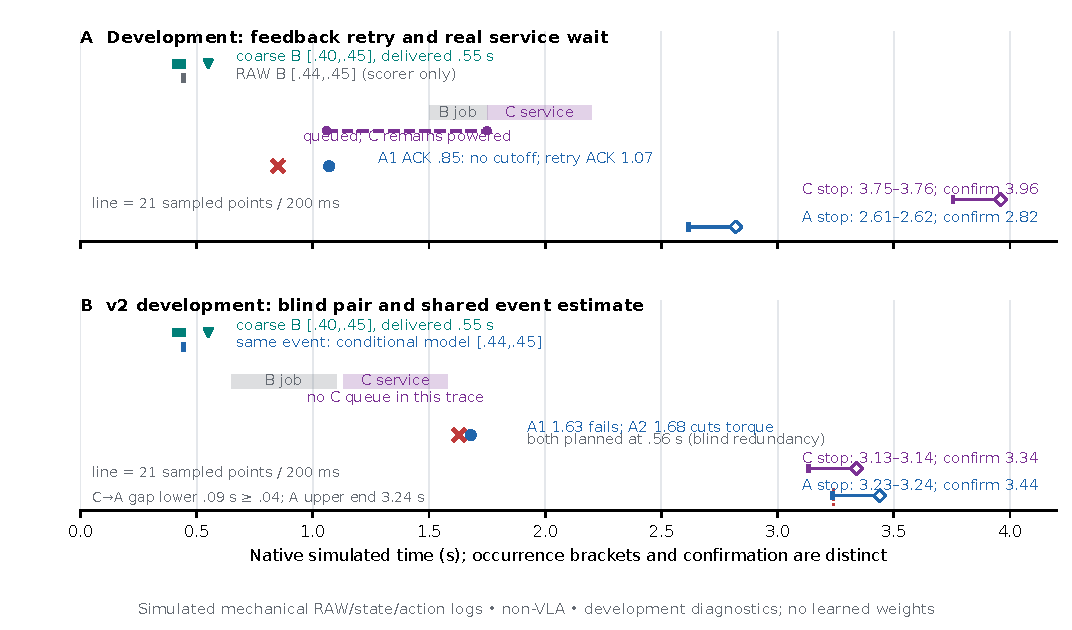
\includegraphics[width=\textwidth]{../../figures/physical_event_timeline_compact.pdf}
\caption{Recorded development timelines: 4.2 s of complete 12 s traces.
A: ineffective ACK, feedback retry and powered C queue. B: same-event
inference and preplanned redundancy. Short marks: occurrence brackets;
open diamonds: 21-point/200 ms confirmation. Simulated mechanical
state/action; no RGB, VLA, hardware or learned-policy claim.}
\label{fig:timeline}
\end{figure*}

\section{Problem and positioning}
Command receipt, physical termination and chemical completion have
different times. MATTERIX already supplies chemistry twins, waiting,
concurrent workflows and process verification, and separates heater-off
from reaction completion \cite{matterix}. Chronos and Time as a Control
Dimension already investigate physical time and punctual control
\cite{chronos,timecontrol}. We ask whether verified recovery experience improves a shared policy
beyond matched-information control and matched-budget data. This
component report does not evaluate that learning claim.

\section{Contracts and causal information}
A task declares predicates, graph, observations and resources.
Occurrence intervals $I_e=[\ell_e,u_e]$ share one epoch. For target $D$,
\[
 I_{\rm err}=[\ell_b-u_a-D,\;u_b-\ell_a-D].
\]
Containment in $[-\epsilon,\epsilon]$ is TRUE; disjointness is FALSE;
partial overlap is UNKNOWN. Missing/invalid events cannot succeed.
Joint scoring requires original references and physical/graph predicates;
refusal, UNKNOWN and exhaustion remain in the episode denominator.

Our CPU MuJoCo fixture contains three contact-free motors. B's first
actual $q=2$ crossing is the original event; nonnegative B torque and
no state/time rewrite make it irreversible under the interface.
A/C torque changes only at ACK; the first A transaction fails physically.
Delayed public packets contain position, velocity, torque, timestamps
and reservations. ACK has no effect-success flag; referee RAW is private.
Public B $[.40,.45]$ s arrives at .55 s. A predeclared nominal model
conditionally estimates the \emph{same} event as $[.44,.45]$ from legal
packets; the coarse record persists. Every baseline may use this model.
Packet compatibility is not model-support certification.

For C's $D\pm\epsilon$, A's upper bound $U_A$, C-to-A gap $g$ and
reference/C/A box widths $w,c,a$, combining lower/upper bounds yields
\[
 w+c+g+a\le U_A-D+\epsilon.
\]
This necessary box condition is not resource feasibility. Two possible
A effects from 50 ms-separated ACKs initially have a roughly 60 ms
union; public torque feedback can select a 10 ms box. Coarse-box refusal
is neither physical impossibility nor an information lower bound.

\section{Diagnostics and three failure classes}
The v2 diagnostic independently crosses graph order, B service
50/450 ms and $D=2.8/3.1$ s: eight fixed configurations, not random seeds.
A must stop $[1.8,D]$ after B, C within $D\pm .15$, with a 40 ms edge.
B's reservation starts at .65 s; declared torque and motion persist
through its event plus six seconds. One public batch allows two A
requests for both none/one-drop hypotheses; redundancy is not diagnosis.

All eight witnesses are joint TRUE: four per graph. Each 12 s trace
has 1,201 RAW samples. Sixteen producer/third-party command replays
match state/time exactly: 24 epochs, 28,824 rows; primary remains eight.
Source was frozen first. Stops require prior
movement and 21 low-speed samples spanning 200 ms. Onset and
confirmation differ; sampled maintenance does not guarantee intervals
between samples. Each witness charges two decision ticks and 282--370 proposals;
host computation otherwise pauses the plant.

\paragraph{Qualification.}
A prior rigid-bottle qualification passes mechanical criteria but has
three EARLY timing scores and FALSE strict sampled hold. Supported
stable release onset cannot become first unloading or a contact fraction.

\paragraph{Reachability.}
The old resource draft retains six unsupported conditions out of eight.
A .75 s candidate still has a high-busy C-to-A counterexample: post-slot
C ends $\ge3.21$ s, but the deadline/edge require $\le3.19$ s; pre-slot
is too early. These drafts are not native trials; .65 s has native witnesses.

\paragraph{Attribution.}
Public-model inference removes the coarse-reference restriction here.
One rule batch solves all eight without queries or training: no agentic
necessity or advantage, and no demonstrated post-failure adaptation.

\section{What a learning claim still needs}
Seen nominal configurations are development data; repeating 32 trials
would compare mechanisms, not unseen tasks. Preserve any null advantage
over strong event/HSM control. Freeze observer/model/harness/gains;
separate weight updates from retained/reset context. Match backbone/data, labels, updates, interactions and compute across
DP/history, offline imitation, DAgger and student-state learning.
Aggregation alone is not distinct OPD. Independently calibrate flow,
loaded RPM, transfer and chemical endpoints; these rotors do not certify
C5/C6/C13. Formal32 trials, fit, GPU, LLM and weight updates here: zero.
Independent review/replay pass; the audit is post hoc, not prospective.

\begin{thebibliography}{9}
\bibitem[Darvish et~al.(2026)]{matterix}
Darvish, K. et~al. MATTERIX: toward a digital twin for robotics-assisted
chemistry laboratory automation.
\emph{Nature Computational Science}, 6:67--82, 2026.
\href{https://doi.org/10.1038/s43588-025-00924-4}{doi:10.1038/s43588-025-00924-4}.
\bibitem[Chronos(2026)]{chronos}
Chronos Policy: Learning Robot Policies on Physical Time.
\href{https://arxiv.org/abs/2610.13929}{arXiv:2610.13929}, 2026.
\bibitem[Time Control(2026)]{timecontrol}
Time as a Control Dimension in Robot Learning.
\href{https://arxiv.org/abs/2511.07654}{arXiv:2511.07654}, version 2, 2026.
\end{thebibliography}
\end{document}
